\section{\ac{lora}}
\label{sec:lora}
\subsection{Overview}
\ac{lora} is a physical long-range, low-power, communication technology developed and patented by Semtech\footnote{Semtech, USA, https://www.semtech.com/}. It is designed to operate inside either the Sub-1GHz or 2.4GHz unlicensed \ac{ism} bands worldwide. Consequently, under the proviso that local regulatory standards are obeyed (see Section \ref{sec:ISMBandRegulation}), it can be used for wide area deployments without being tied to expensive licensed carriers. Fundamentally, even using its fastest configuration, it is a low-data rate modulation technique.

Long-range communication can be a challenge in the \ac{ism} bands as the heavy congestion can result in a high physical noise floor. That is the sum of all signals in the band from sources such as the atmosphere or radio devices, excluding that of the signal being monitored. \ac{lora} functions using a unique spread spectrum modulation technique that can operate below the noise floor. Spread spectrum techniques allow signal-to-noise degradation in a single channel to be compensated for by spreading across other channels. Unlike other spread spectrum techniques that use a fixed chip sequence to carry out spreading, \ac{lora} modulation uses a chirp signal that varies in frequency continuously. This is referred to as chirp spread spectrum (\ac{css}) modulation and allows the complexity of the receiver design to be greatly reduced, resulting in a reduced and accessible hardware cost \cite{3YP:LORA_MOD_BASICS}. 

The link budget of a \ac{rf} system is defined as the measure of all gains and losses incurred by a signal passing through the transmitter, the receiver and the propagation channel. The equation in its simplest form is:
\begin{equation}
\label{eq:link_budget}
RX\ Power\ (dB)\ = TX\ Power\ (dB)\ +\ Gains\ (dB)\ -\ Losses\ (dB)
\end{equation}
A system is said to be link limited when the channel losses result in a receive power (and therefore \ac{snr}) lower than can be demodulated by the receiver. \ac{lora} modulation boasts a high and adapative receiver sensitivity compared to frequency shift keying (FSK) and other modulation types, allowing it to make far more efficient use of its link budget \cite{3YP:LORA_MOD_BASICS}.

\subsection{Parameters}
\ac{lora} hardware has many parameters that can be configured to extend range or increase reliability at the expense of air time, data-rate or energy consumption. These are independent from any external hardware and include:
\begin{itemize}
    \item \textbf{Bandwidth (\ac{bw})}: The range of the chirps around the \ac{cf}. Increasing bandwidth increases data-rate but decreases receiver sensitivity \cite{3YP:STUDY_OF_LORA}.
    \item \textbf{Carrier Frequency (\ac{cf})}: The centre frequency of chirps. Current hardware targets some sub-range of 137MHz to 1020MHz at a resolution of 61Hz \cite{3YP:LORA_SX12}. 
    \item \textbf{Coding Rate (\ac{cr})}: The amount of redundant information encoded in symbols for forward error correction (\ac{fec}); trade-offs can be seen in Table \ref{cr_effect}. \ac{fec} is most effective in the presence of burst interference \cite{3YP:LORA_MOD_BASICS}.
    \item \textbf{Preamble Symbols (\ac{ps})}: The number of programmed preamble symbols sent for receiver synchronisation. Packet receive percentage (\ac{prp}) has been shown to increase with an increased \ac{ps} up to a certain threshold \cite{3YP:LORA_PERFORMANCE}. Increasing length can also improve performance of \ac{cad} (see Section \ref{sec:cad}).
    \item \textbf{Spreading Factor (\ac{sf})}: The ratio of chip rate to bit rate, where chips per symbol is given as $2^{\text{\ac{sf}}}$. Receiver sensitivity increases in line with spreading factor and is therefore a factor in the link budget \cite{3YP:LORA_SX12}. The trade-offs can be seen in Table \ref{sf_effect}.
    \item \textbf{Transmission Power (\ac{tp})}: The radio output power. Equation \ref{eq:link_budget} highlights how an increased \ac{tp} directly increases link budget with the obvious drawback of higher power usage. 
\end{itemize}


\begin{table}[H]
\centering\small
\caption[Effect of \ac{cr}s on \ac{lora} transmissions]{Effect of \ac{cr}s on \ac{lora} transmissions. Recovery performance is defined as the best case percentage of bits that can be lost for a successful receive. \\ Compiled from data in \cite{3YP:LORA_PERFORMANCE}.}
\label{cr_effect}
\begin{tabular}{c|cc}
    \toprule
    \textbf{Coding Rate} & \textbf{Data Overhead} & \textbf{Recovery}  \\
    \midrule\addlinespace
    4/5 & $\times$1.25 & 20\% \\
    4/6 & $\times$1.50 & 33\% \\
    4/7 & $\times$1.75 & 43\% \\
    4/8 & $\times$2.00 & 50\% \\
    \addlinespace\bottomrule
\end{tabular}
\end{table}
\begin{table}[H]
\centering\small
\caption[Effect of \ac{sf} on \ac{lora} transmissions]{Effect of \ac{sf} on \ac{lora} transmissions (\ac{bw}=125KHz). \\Compiled from data in \cite{3YP:LORA_MOD_BASICS} and \cite{3YP:LORA_PERFORMANCE}.}
\begin{tabular}{c|ccc}
    \toprule
    \makecell{\textbf{\ac{sf}} \\ \textbf{(\ac{lora} Mode)}} & \makecell{\textbf{\ac{sf}} \\ \textbf{(Chips / Symbol)}} & \makecell{\textbf{Bit Rate} \\ \textbf{(bits / sec)}} & \makecell{\textbf{Demodulation Limit} \\ \textbf{(\ac{snr} dBm)}} \\
    \midrule\addlinespace
    SF7 & 128 & 5469 & -7.5 \\
    SF8 & 256 & 3125 & -10.0 \\
    SF9 & 512 & 1758 & -12.5 \\
    SF10 & 1024 & 977 & -15.0 \\
    SF11 & 2048 & 537 & -17.5 \\
    SF12 & 4096 & 293 & -20.0 \\
    \addlinespace\bottomrule
\end{tabular}
\label{sf_effect}
\end{table}
\label{sec:parameter_selection}
Selection of these parameters is often manual, however mechanisms such as \ac{lorawan}'s adaptive data-rate (\ac{adr}) \cite{3YP:LORAWAN}, or ``probing algorithms'', as proposed by \cite{3YP:CHOOSING_LORA_PARAMETERS}, can be used to choose these parameters such that transmission energy is reduced whilst maintaining an adequate throughput and link budget. \ac{lorawan} abstracts \ac{sf}s and \ac{bw}s into a set of orthogonal data-rates (\ac{dr}s) to simplify selection, where lower data-rates have higher range \cite{3YP:LORAWAN_REGIONAL_PARAMS}. It has been suggested that \ac{adr} has low-scalability due to packet count requirements \cite{3YP:LORAWAN_ADR} and is slow to converge \cite{3YP:LORAWAN_ADR_AGILITY}. Likewise \cite{3YP:CHOOSING_LORA_PARAMETERS} requires a large number of initial transmissions, making both only suitable for static nodes in a gateway controlled network.

\subsection{Airtime}\label{sec:airtime}
To understand a configuration's performance, it is critical to know its airtime; this defines bitrate and affects channel contention methods. The total airtime of a transmission (Equation \ref{eq:airtime}) is dependent on the number of symbols being transmitted (Equation \ref{eq:symbol_count}) and the time each symbol takes to send. Preamble and payload are calculated individually as it can be useful to consider them as separate components for purposes such as \ac{cad}. Equations are adapted from \cite{3YP:LORA_SX12} to suit the notation and formats used by this paper.
\begin{subequations}
\label{eq:symbol_count}
\begin{align}
	S_{preamble} &= \text{\ac{ps}} + 4.25 \\
	S_{payload} &= 8 + \max\left( \text{ceil}\left[ \frac{8\text{\ac{pl}}-4\text{\ac{sf}}+16\text{\ac{crc}}+20\text{\ac{eh}}+8}{4(\text{\ac{sf}}-2\text{LDR})}\right] \frac{1}{\text{\ac{cr}}},\enskip 0\right) \\
	S_{total} &= S_{preamble} + S_{payload} 
\end{align}
\end{subequations}

The unmentioned factors in Equation \ref{eq:symbol_count} are: the number of bytes in the packet (\ac{pl}), whether the \ac{crc} check is enabled (0 or 1), whether the explicit header (\ac{eh}) is enabled (0 or 1) and whether low-data-rate optimisation (LDR) is enabled (0 or 1). LDR is used when $T_s > 16ms$ to aid stability over long transmits \cite{3YP:LORA_SX12}.
\begin{subequations}
\label{eq:airtime}
\begin{align}
	T_{s} &= \frac{1}{S_R} = \frac{2^{\text{\ac{sf}}}}{\text{\ac{bw}}}\label{eq:symbol_time} \\
	T_{preamble} &=  S_{preamble}\cdot T_{s}\\
	T_{payload} &= S_{payload}\cdot T_{s} \\
	T_{a} = T_{packet} &= T_{preamble} + T_{payload}
\end{align}
\end{subequations}

Equation \ref{eq:airtime} highlights that each \ac{sf} increment will cause $T_a$ to double for the same  number of symbols. Likewise, doubling \ac{bw} will half $T_a$. Figure \ref{lora_transmission_structure} shows the structure of a \ac{lora} transmission and therefore where each airtime component comes from. 

\begin{figure}[H]
    \centering
   	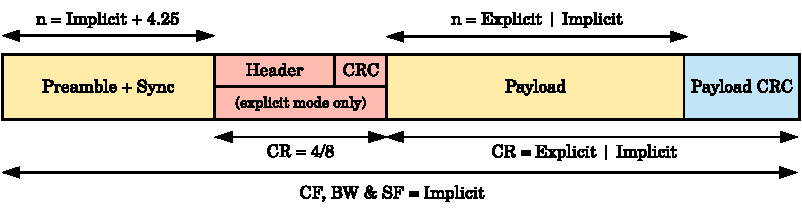
\includegraphics{Figures/lora_transmission.pdf}
    \caption[\ac{lora} transmission packet structure]{
    Structure of a standard \ac{lora} transmission. All transmissions contain a preamble, sync words, and a payload. The header section (in red) is optional but if present, contains information such as the payload length, the payload \ac{cr}, and whether the \ac{crc} is present. If the header is not present this information must be fixed implicitly by the receiver. Parameters that are not in the header are always implicit and must match between transmitter and receiver (i.e. \ac{pl}, \ac{sf}, \ac{bw} and \ac{cf}). Adapted from \cite{3YP:LORA_SX12}.
    }
    \label{lora_transmission_structure}
\end{figure}


\subsection{Receive Behaviour}
\label{sec:lora_considerations}
\ac{lora} radios, like all current consumer radios, are half-duplex, meaning that they are unable to receive for the duration of transmissions. Additionally, end device radios will usually be transceivers, which can only demodulate one incoming signal at a time \cite{3YP:LORA_SX12}. In the presence of multiple signals, some transmissions may be missed, or collisions may occur, causing all transmissions to be missed. Collision scenarios specific to \ac{lora} are identified in Table \ref{tab:collisions}. 

\begin{table}[H]
\centering\small
\caption[\ac{lora} collision scenarios]{Collation of \ac{lora} collision scenarios as defined by \cite{3YP:LORA_FOR_IOT} and \cite{3YP:LORA_COLLISIONS}. \cite{3YP:LORA_COLLISIONS}'s definition of the important preamble (IP) is used: the four fixed preamble symbols and proceeding two symbols of the programmed preamble. Situations use two transmission sources (A and B) and one receive source (C).}
\begin{tabular}{c|cc|c}
    \toprule
    \textbf{ID} & \textbf{Time} & \textbf{Power} & \textbf{$C$ Result}\\
    \midrule\addlinespace
    A & $B_{start} > A_{\text{IP}}$ & $A_{\text{\ac{rps}}} \geq B_{\text{\ac{rps}}}$ & Receives A \\
    B & $B_{start} > A_{\text{IP}}$ & $A_{\text{\ac{rps}}} < B_{\text{\ac{rps}}}$ &  Receives A \\
    C & $B_{start} > A_{\text{IP}}$ & $A_{\text{\ac{rps}}} \ll B_{\text{\ac{rps}}}$ & CRC Fail A \\
    D & $B_{start}$ \textit{inside} $A_{\text{IP}}$ & $A_{\text{\ac{rps}}} \leq B_{\text{\ac{rps}}}$ & Collision \\
    E & $B_{\text{IP}} \approx A_{\text{IP}}$ & $A_{\text{\ac{rps}}} \approx B_{\text{\ac{rps}}}$ & Collision \\
    F & $B_{\text{IP}} \approx A_{\text{IP}}$ & $A_{\text{\ac{rps}}} \gg B_{\text{\ac{rps}}}$ & Receives $A$ \\
    \addlinespace\bottomrule
\end{tabular}
\label{tab:collisions}
\end{table}

 It should be noted that a different technology exists in gateways (a \ac{lora} concentrator block), allowing demodulation of up to eight signals concurrently, provided they use unique spreading factors \cite{3YP:LORA_SX1301}. Although gateways are clearly more powerful than transceivers, their cost and power usage make them hard to deploy on scale. However, Pycom's\footnote{Pycom, UK,  https://pycom.io/} newly released Pygate gateway is a fraction of the cost of existing implementations and may be feasible for ad-hoc scenarios.

 Most \ac{lora} applications consist of many sensor nodes infrequently sending data on different spreading factors to a single gateway with very little downlink present; this means collisions and missed receives are rare. Unfortunately, in ad-hoc networks, these events are very likely and can be detrimental to a network's throughput; this is further explored in Section \ref{sec:mac_protocol_background}.
\newpage
\subsection{Channel Activity Detection (\ac{cad})}\label{sec:cad}
Carrier-sensing is a helpful mechanism for radios to check whether a channel is busy or idle. Usually, this is achieved by checking the power present in the channel using the received signal strength indicator (\ac{rssi}). This is a very unreliable method for \ac{lora} because the \ac{rssi} includes channel noise, and \ac{lora} signals can operate below the noise floor. For this reason, \ac{lora} radios offer a specialised \ac{cad} method, which searches the channel for a single \ac{lora} packet preamble symbol. \ac{cad} is at least 97\% reliable in the presence of preamble with false positives occuring just 0.1\% of the time \cite{3YP:LORA_FOR_IOT}. It has been shown that \ac{cad} can in fact detect non-preamble symbols when there is high signal strength, although this ability quickly becomes unreliable in a real world scenario \cite{3YP:LORA_CSMA}.

\subsection{Signal Orthogonality}\label{sec:sf_orthogonality}
The manner of \ac{lora}'s modulation allows multiple signals to co-exist in the same channel provided they have a different chirp rate, where $C_R = \text{\ac{bw}} \cdot S_R$, otherwise written as $C_R = \frac{\text{\ac{bw}}^2}{2^{\text{\ac{sf}}}}$. This clearly demonstrates that for a single bandwidth, all \ac{sf}s must be orthogonal to one another. However, in the case that different \ac{bw}s are used, different \ac{sf}s may have the same chirp rate and could interfere; this is demonstrated in Figure \ref{fig:orthogonality}.

\begin{figure}[H]
    \centering
   	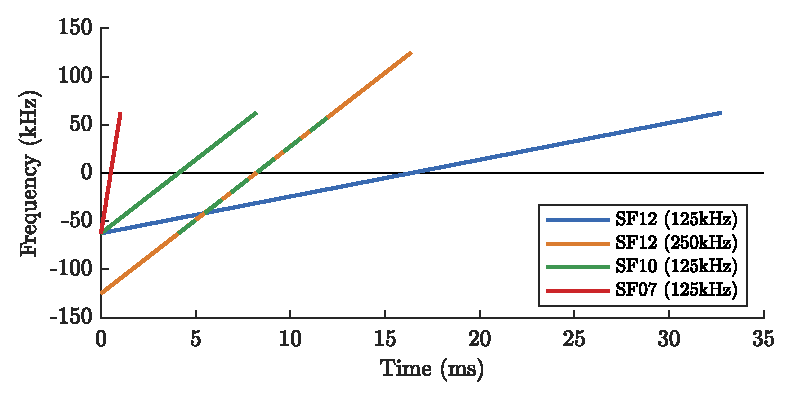
\includegraphics{Figures/sf_orthogonality_plot.eps}
    \caption[Signal chirp rate orthogonality]{
    Demonstration of signal orthogonality for different \ac{sf}s. The SF10 (125kHz) chirp is duplicated and shifted to overlap with the  SF12 (250kHz) chirp to highlight that they have the same chirp rate and are therefore not orthogonal.
    }
    \label{fig:orthogonality}
\end{figure}
%Symbol duration is the inverse of the symbol rate, defined in \ref{cr_effect}

